\chapter{Agglomerative clustering algorithms}

Clustering analysis --- or clustering --- is a reduction of a complex object group into several small, less complex disjunctive subgroups. The reduction is performed in such way that objects from one subgroups share a common property (i.e. they are mutually compatible, or similar). Hence, clustering is used to identify and extract significant partitions from the underlying data. 

In the field of clustering analysis, there is no strict definition for a cluster itself. That may be one reason why there is such a vast amount of clustering algorithms; many authors such as \citet{estivill2002so} discuss this topic.  Despite the lack of the definition, the~one common property that we can find among all the algorithms is the presence of a~group of data objects.

Depending on a field of use, the data objects are represented variously (as graphs, text sequences, etc.). The current thesis will focus on a clustering of objects represented by a vector of real numbers.

Suppose a dataset $\mathcal{D}$ given as a $n$ $d$-dimensional vectors $(x_1,\dots,x_d) \subset \R^d$  --- objects; each element of a vector describes a specific object property. Two objects are similar if values of their respective properties are alike. Then, a clustering analysis can be defined as a form of an object grouping into subsets of $\mathcal{D}$ that maximizes the inter-set object similarity and minimizes the intra-set object similarity.

\section{Clustering models}

Specific variations of clustering analysis are defined by a clustering model. There is a great amount of them, since their field of use varies. For the~purpose of the following chapters, we first describe the \emph{centroid-based model}. Then, we fully focus on the \emph{hierarchical model}. 

Since the current thesis focuses on the clustering of vectors of real numbers, we define the following terms and establish the terminology:

\begin{defn}[Vector-space dataset]
	Given the real vector space $\R^d$, an input of clustering analysis $\mathcal{D}\subset\R^d$ is called the \emph{vector-space dataset}.
\end{defn}

\begin{defn}[Cluster]
	Given a vector-space dataset $\mathcal{D}$, we define the \emph{cluster} $C$ of $\mathcal{D}$ as any subset of $\mathcal{D}$.
\end{defn}

\begin{defn}[Centroid]
	Given a vector-space dataset $\mathcal{D}\subset\R^d$ and its cluster $C$, we define the \emph{centroid} of $C$ as a point in $\R^d$ such that its $i$-th element is equal to the arithmetic mean of the $i$-th elements of all points $o \in C$. We will denote it by $\mean(C)$.
	\label{def01:centr}
\end{defn}

\subsection{Centroid-based model}

The centroid-based clustering model represents clusters only by a central vector --- a centroid --- which is not necessarily a member of a dataset. Further on in the thesis, we will refer to the cluster as to a subset 

Many~implementations of this model need the number of required centroids in advance (denoted by $k$). We define the following optimization problem for~this kinds of~algorithms:

\begin{problem}[Centroid-based clustering]
	Having a distance function $d$, find $k$ centroids $c_1,\dots,c_k$ from the domain of the dataset $\mathcal{D}$ such that the sum \ref{eq01:sum}
	is minimized.
\end{problem}

\begin{equation}\label{eq01:sum}
	\sum_o^{\mathcal{D}} \min_{i=1\dots k}d(o,c_i)
\end{equation}

This problem is difficult to solve; in the euclidean space, the problem is NP-hard~\cite{aloise2009np}. Hence, many approximation algorithms emerged. 

\subsubsection{k-means}

The most common implementation of a centroid-based clustering is \emph{k-means}. Its algorithm can be expressed in a few simple steps (see alg.~\ref{alg01:kmeans}).

\begin{algorithm}[t]
	\caption{$k$-means clustering}
	\label{alg01:kmeans}
	\begin{algorithmic}[1]
		\Procedure{$k$-means}{$k\in\R$, $\mathcal{D} \subset \R^d$, $d \in \R^d \times \R^d \to \R$}
		\State $C \gets$ first $k$ objects from  $\mathcal{D}$ \Comment{select initial centroids}
		\Repeat
			\State $\forall i \in \{1\dots k\}:K_i \gets \{\}$  \Comment{create empty clusters}
			\State $\forall o \in \mathcal{D}:K_{j} \gets K_{j} \cup o$ for such $j$ that $d(C_j,o)$ is minimal \Comment{assign objects to clusters}
			\State $C' \gets \{\mean(K_1),\dots,\mean(K_k)\}$\Comment{compute new centroids}
			\State swap $C$ and $C'$
		\Until{$C = C^\prime$}
		\State \textbf{return} $C$
		\EndProcedure
	\end{algorithmic}
\end{algorithm}


The algorithm divides data into $k$ clusters in an iterative manner. Before the first iteration, initial $k$ central vectors are selected from the~dataset (we chose the first $k$ objects; however, the way of selecting $k$ initial vectors varies between 
implementations). In the iteration loop, dataset objects are grouped into clusters according to the closest centroid (also called the cluster mean; hence, $k$-means). After that, new centroids are computed from new clusters. Next iteration follows until centroids does not change or a predefined number of iterations is reached. 

Since the only performance demanding parts of the $k$-means algorithm are the assignment of points to clusters and the centroid computation, the algorithm is simple and fast. However, it is unable to deal with the noise in~a~dataset and clusters of a non-convex shape~\cite{uppada2014centroid}.
  

\subsection{Hierarchical model}
\label{sec01:hierarch_clust}

In the hierarchical clustering model, objects are connected together forming a tree-like structure. In contrast with the aim of a centroid-based model that returns only $k$ centroids, hierarchical clustering analysis (HCA) captures the whole connecting process. HCA algorithms start with all objects from a dataset as initial clusters. Each iteration, two clusters are connected creating a new one, finishing with one all-inclusive cluster. Commonly, the algorithms represent the connecting process as an ordered list of pairs --- a list of connected clusters~\cite{karypis1999chameleon}.

The result of a hierarchical clustering can be viewed as a \emph{dendrogram} (see fig.~\ref{fig01:dendro}). The y-axis states the measure of similarity between connected clusters. The x-axis shows labels of the objects from a dataset. Hence, the clusters that are connected in the higher part of the dendrogram are considered less similar, and the clusters connected at its bottom are more similar. 

\begin{figure}[t]
	\centering
	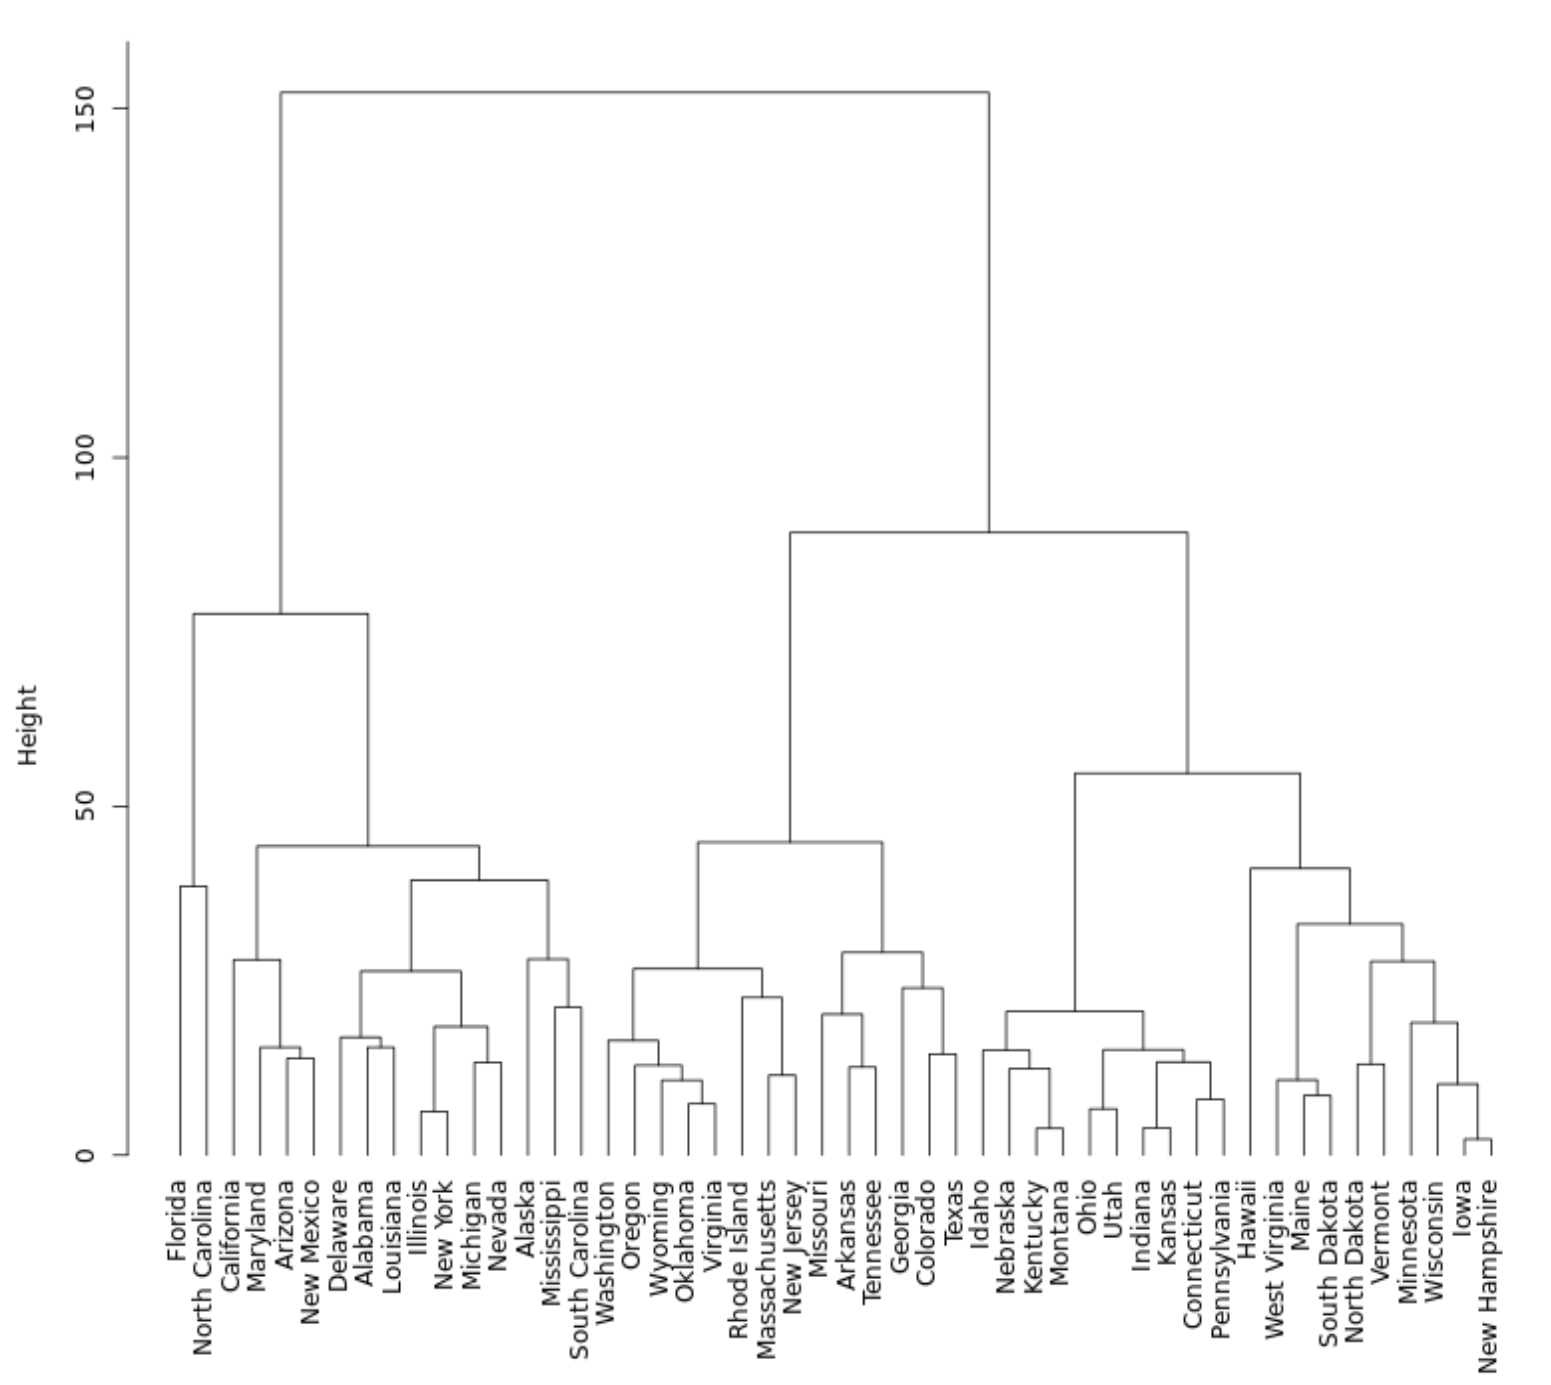
\includegraphics[width=10cm]{img/dendro}
	\caption{An example of a dendrogram; a plant growth under different treatment conditions (R dataset \texttt{PlantGrowth}).}
	\label{fig01:dendro}
\end{figure}

Hierarchical algorithms use two approaches on how to create a dendrogram; \emph{agglomerative} and \emph{divisive}. An agglomerative hierarchical algorithm begins with each object representing a cluster on its own. Then, in a bottom-up fashion, clusters are successively connected into the only cluster. The divisive algorithm begins with a single all-inclusive cluster which is divided into sub-clusters until single objects remain~\cite{rokach2005clustering}. 



To know which two clusters are connected (or respectively, how a cluster is~divided into two), algorithms use a \emph{dissimilarity measure} between clusters.  

\begin{defn}[Dissimilarity measure]
	Given a vector-space dataset $\mathcal{D}\subset\R^d$,  we define the \emph{dissimilarity measure} as the pair $(M,L)$. $M$ is a metric over $\R^d$ and $L$ is a linkage criterion; a function that can measure dissimilarity of subsets of $\R^d$ using $M$. They are used to measure the dissimilarity of clusters during a $\mathcal{D}$ clustering.
\end{defn}

A~hierarchical clustering model distinguishes various kinds of algorithms based on~the~choice of a metric and a linkage criterion. A \emph{distance function} can serve as a metric in a dissimilarity measure:

\subsubsection{Distance functions}

A distance function is used on objects of a dataset to measure how far they are from each other in the observed domain. For objects from a vector-space dataset, variations of \emph{Minkowski distance formula} (see eq.~\ref{eq01:mink}) can be used to easily create the metric for a dissimilarity measure.
They are \emph{Manhattan distance} ($p=1$), \emph{Euclidean distance} ($p=2$) and \emph{Chebyshev distance} ($p \to \infty$) (see tab.~\ref{tab01:mink}). The other possible metric is the \emph{cosine similarity} (see eq. \ref{eq01:cos}).

\begin{equation}\label{eq01:mink}
||a-b||_p = (\sum_{i=1...d}|a_i-b_i|^p)^{\frac{1}{p}}
\end{equation}

\begin{equation}\label{eq01:cos}
cos(a,b) = \dfrac{a\cdot b}{||a||||b||}
\end{equation}

As the choice of a distance function influences the result of a clustering, it should be chosen with respect to the properties of a provided dataset. \citet{aggarwal2001surprising} show the qualitative behavior of different distance functions in the $k$-means algorithm.



\begin{table}[t]
	\centering
	\renewcommand{\arraystretch}{1.3}
	\begin{tabular}{ll}
		\toprule
		Distance measure & Formula \\
		\midrule
		Manhattan & $\|a-b\|_1 = \sum_{i}|a_i-b_i|$          \\
		Euclidean & $\|a-b\|_2 = \sqrt{\sum_{i}(a_i-b_i)^2}$ \\
		Chebyshev & $\|a-b\|_\infty = \max_{i}|a_i-b_i|$  \\
		\bottomrule
	\end{tabular}
	\caption{Variations of the Minkowski distance formula.}
	\label{tab01:mink}
\end{table}

\subsubsection{Linkage criteria}

A~hierarchical algorithm can not compute the dissimilarity of two clusters only by a distance function; it is a function of dataset objects. To completely define the dissimilarity measure, we need a function of sets of object --- a linkage criterion. It describes any process of measuring dissimilarity between two groups of objects. In a hierarchical algorithm, it measures clusters to determine which two will be linked together. Given clusters $A$ and $B$ of a vector-space dataset and a distance function~$d$, we define the following linkage criteria~\cite{yim2015hierarchical} (see fig.~\ref{fig01:link}):

\begin{description}
	\item[Single linkage] -- The single linkage criterion computes the distance between $A$ and $B$ as the minimum distance between all pairs $(a,b) \in A\times B$:
	$$\min\{d(a,b) : a \in A, b \in B\}.$$
	
	The major drawback this criterion suffers is the \emph{cluster chaining}. It occurs when connected clusters do not share any other pair of close objects than the one that determined the connection. This produces long thin clusters with a big distance between some objects.
	
	\item[Complete linkage] -- The complete linkage criterion is similar to the single linkage criterion. But as opposed to~finding the minimum, this criterion uses the maximum of object pairs for the~computation of a cluster dissimilarity:
	$$\max\{d(a,b) : a \in A, b \in B\}.$$
	
	The criterion suffers from its simplicity as well as the single linkage. But~instead of naively connecting dissimilar clusters, here similar clusters are~not connected in some cases. Having all object pairs in a close proximity to each other but one object being rather far from the others, the~criterion will not link the clusters as the maximum distance deteriorates the rest.
	
	\item[Centroid linkage] -- The centroid linkage criterion tries to solve the problems of~the~aforementioned criteria by measuring the distance between the centroids of clusters. It~introduces a form of an average into the computation; the think that the criteria above lack.
\end{description}

The choice of a linkage criterion in hierarchical clustering algorithm is vital. As~stated above, it can change the course of clustering in a great manner. Chosen improperly, it can have a disastrous effect on the final result.

\begin{figure}\centering
	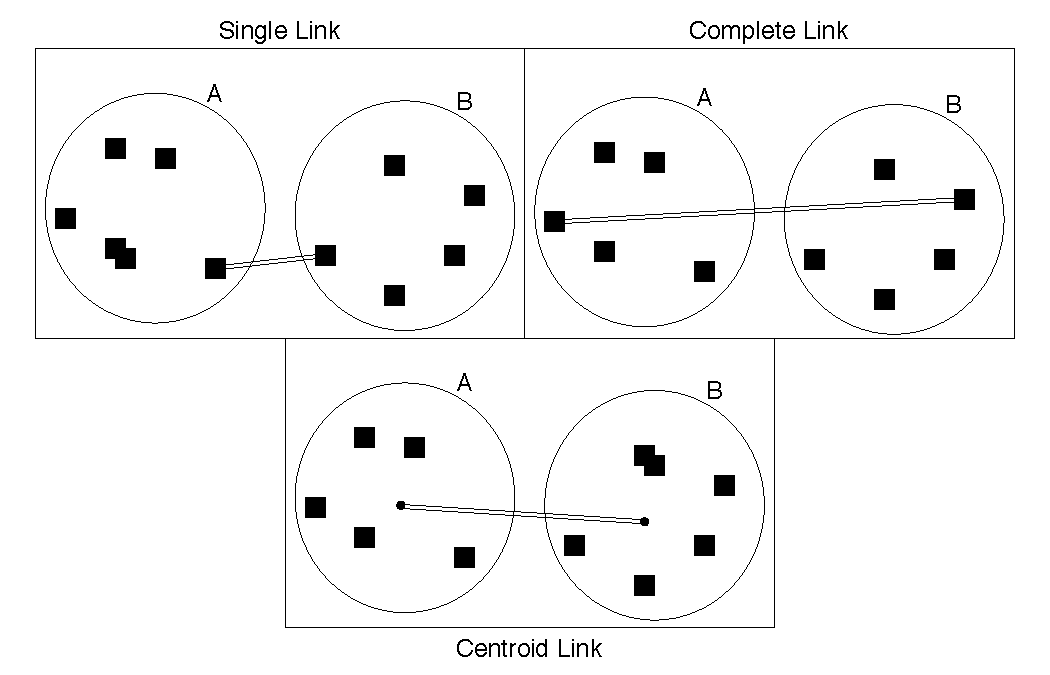
\includegraphics[width=10cm]{img/linkage_criteria}
	\caption{An example of three linkage criteria. The double line represents the~distance between clusters A and B according to the respective criterion.}
	\label{fig01:link}
\end{figure}

\section{Hierarchical clustering with the Ma\-ha\-la\-no\-bis linkage}

Commonly, HCA algorithms branch into different variations so they are more suitable for a specific dataset type~\cite{murtagh2008hierarchical,oh2004hierarchical,zhao2005hierarchical}. A common cause for such customization is a shape of clusters, i.e. an elliptical or gaussian shape (see fig. \ref{fig01:mhca}). A general HCA is unable to properly cluster such dataset. The~\emph{Ma\-ha\-la\-no\-bis-average hierarchical clustering analysis} (MHCA) focuses on the datasets that create clusters of ellipsoid shapes. Such datasets commonly originate in the~measurements of cell cytometry data in bioinformatics, which was the original purpose for the design of MHCA.

\begin{figure}[t]\centering
	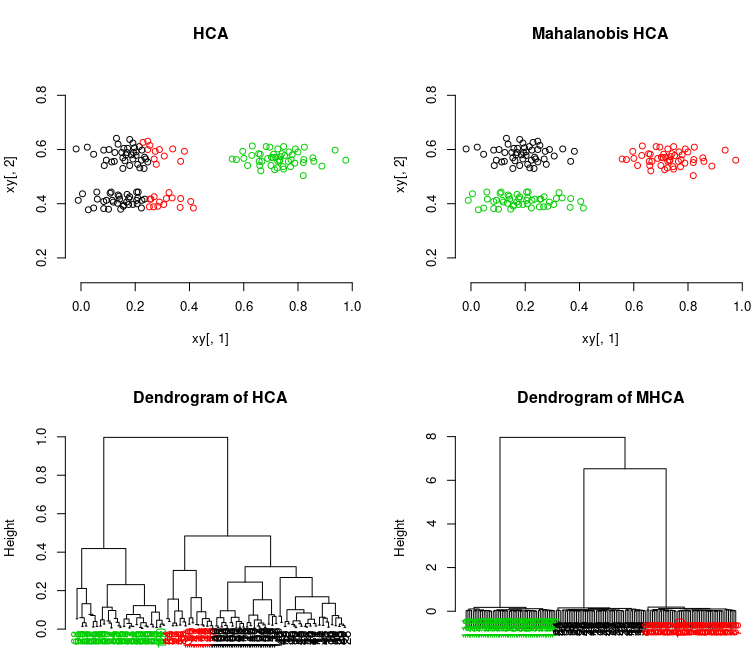
\includegraphics[width=10cm]{img/mhca}
	\caption{A comparison of HCA and MHCA clustering on a dataset that contains elliptic groups of points (taken from the \texttt{tsieger/mhca} Github repository). The upper two figures show the state of clustering when both algorithms cluster the dataset into three clusters. MHCA properly recognizes the elliptic clusters.}
	\label{fig01:mhca}
\end{figure}

\subsection{Mahalanobis distance}

An important part of MHCA is the dissimilarity measure based on the \emph{Mahalanobis distance}~\cite{mahalanobis1936generalized}, a~distance between a~point and a set of points (in our case a cluster). If points in the set are strongly correlated in some axis, then points laying on this axis are closer to the set than points that are not; even if their euclidean distance to the center of the set is closer.

To measure the Mahalanobis distance, a covariance matrix of~a~participating cluster needs to be computed. We compute the covariance matrix using the random vector of a cluster.

\begin{defn}[Random vector of a cluster]
	Given a cluster $C$ of a vector-space dataset, we define its \emph{random vector} $v$ as a vector of $d$ discrete random variables, where the random variable $v_i$ takes values from $\{x_i:x\in C\}$ with equal probability.
\end{defn}

\begin{defn}[Covariance matrix]
	Given a random vector $v$ of length $n$, we define the \emph{covariance matrix} $\cov(v)$ as a $n\times n$ matrix that holds covariances of each pair of vector element:
	$$\cov(v)_{i,j}=\cov(v_i,v_j)$$
\end{defn}

Using the random vector of a cluster we can compute the covariance matrix of a cluster and properly define the Mahalanobis distance:

\begin{defn}[Mahalanobis distance]
	Suppose a cluster $C$ of a vector-space dataset $\mathcal{D}\in\R^d$ and the random vector $v$ of $C$. If the $\cov(v)$ is regular, we define the \emph{Mahalanobis distance} between $u \in \R^d$ and $C$ as
	\begin{equation}
	d_\text{Maha}(u,C) = \sqrt{(u-\mean(C))^T\cov(v)^{-1}(u-\mean(C))}.
	\end{equation}\label{eq01:maha}
\end{defn}

Note that this equation computes a distance between a point and a cluster. To fully incorporate the Mahalanobis distance in a hierarchical algorithm, we need to construct a method to measure a distance between two clusters.

Two usable methods naturally arise. We compute either the arithmetic mean of the distances between all points and a cluster or just the distance between a centroid and a cluster. We respectively call these methods the \emph{Full Mahalanobis distance} (FMD) and the \emph{Centroid Mahalanobis distance} (CMD).

\begin{defn}[Full Mahalanobis distance]
	Having clusters $C$ and $C'$, we define the \emph{Full Mahalanobis distance} between clusters $C$ and $C'$ as the arithmetic mean of the Mahalanobis distances between each object $o \in C$ and the~cluster $C'$:
	$$d_\text{MahaFull}(C,C') =\frac{1}{|C|}\sum_{o\in C}{d_\text{Maha}(o,C')}$$
	\label{def01:fmd}
\end{defn}

\begin{defn}[Centroid Mahalanobis distance]
	Having a cluster $C$ with its centroid $c$ and a cluster $C'$, we define the \emph{Centroid Mahalanobis distance} between clusters $C$ and $C'$ as the Mahalanobis distance between $c$ and $C'$:
	$$d_\text{MahaCentroid}(C,C')=d_\text{Maha}(c,C')$$
	\label{def01:cmd}
\end{defn}


To illustrate the measure of the Mahalanobis distance, let us suppose we have two elliptic clusters. In the means of the proximity, the measure favors such clusters that their ellipsis are alongside rather than in a prolongation of one another~\cite{dagnelie1991using} (see fig.~\ref{fig01:ellipses}). Only when the objects of a cluster form a spherical shape, this measure of dissimilarity is proportional to the euclidean distance with a corresponding linkage.

\begin{figure}\centering
	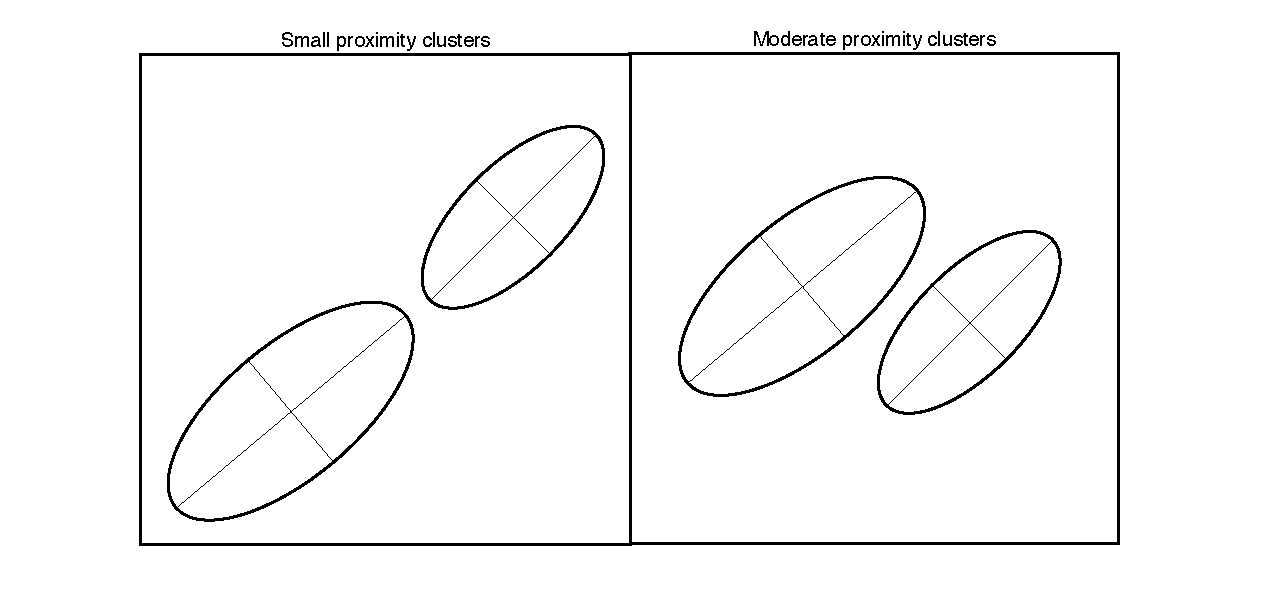
\includegraphics[width=10cm]{img/ellipses}
	\caption{An example of the cluster dissimilarity in the Mahalanobis-average hierarchical clustering.}
	\label{fig01:ellipses}
\end{figure}


CMD can be interpreted as an approximation substitute for FMD variant. A case when CMD variant fails to compute good approximate measure happens when centroids of measured clusters are very close to each other while their points do not lay on each others major axis (see fig.~\ref{fig01:maha_var}). Such case is rather unrealistic; therefore, we assume it is unlikely to happen in cell cytometry datasets.

\begin{figure}\centering
	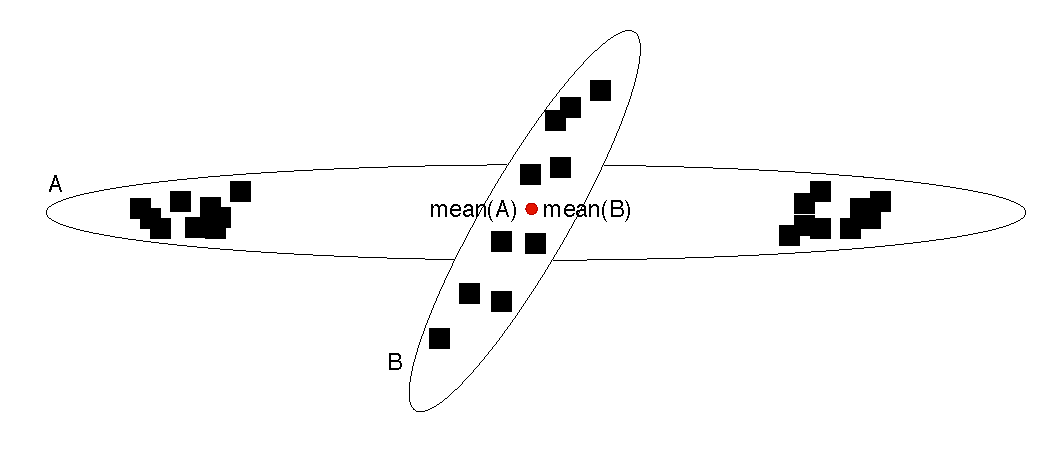
\includegraphics[width=10cm]{img/maha_variant}
	\caption{An example of clusters with a big difference between FMD and CMD dissimilarity measures.}
	\label{fig01:maha_var}
\end{figure}

To properly utilize the Mahalanobis distance variants as dissimilarity metrics in a MHCA implementation, we need the distance function to be symmetric. Originally, the Mahalanobis distance is not a symmetric function. Fortunately, we easily fix the aforementioned distance functions with the Generalized distance.

\begin{defn}[Generalized distance]
	Given clusters $C$, $C'$ and a variant of the Mahalanobis distance~$d_\text{Variant}$ (either FMD or CMD), we define the \emph{Generalized distance} between clusters $C$ and $C'$ as the arithmetic mean of distances between $C$, $C'$ and $C'$, $C$:
	$$d_\text{General}(C,C') = \frac{d_\text{Variant}(C,C')+d_\text{Variant}(C',C)}{2}$$
	\label{def01:gene}
\end{defn}  


\subsection{Singularity of cluster covariance matrix}

In early stages of MHCA --- when clusters consist of fewer points --- the covariance matrix of a cluster is often singular As a result, we can not compute its inverse and perform the distance measure. Furthermore, the matrix can happen to be close to singular and --- when inverted --- can produce false results such as negative distances or infinity floating points.

To solve this problem, \citet{fivser2012detection} specified a cluster size threshold; if the size of a cluster is lower than the threshold, then the cluster dissimilarity measurements are computed using euclidean distance. The value of the threshold is proportional to the size of a dataset. We denote this threshold as the \emph{Mahalanobis threshold} and to implement the singularity workaround we defined the Non-singular Mahalanobis Distance.

\begin{defn}[Non-singular Mahalanobis Distance]
	Given a threshold $T_M$, a cluster $C$ and its centroid $c$, a cluster $C'$ and its centroid $c'$ and a variant of the Mahalanobis distance~$d_\text{Variant}$ (either FMD or CMD), we define the \emph{Non-singular Mahalanobis Distance} as
	$$
	d_\text{NSing}(C,C')=
	\begin{cases}
		d_\text{General}(C, C'),                       & \text{if $|C|\ge T_M$ and $|C'|\ge T_M$}, \\
		\dfrac{d_\text{Variant}(C, C')+||c-c'||_2}{2}, & \text{if $|C| < T_M$ and $|C'|\ge T_M$},  \\
		\dfrac{||c-c'||_2+d_\text{Variant}(C', C)}{2}, & \text{if $|C|\ge T_M$ and $|C'|< T_M$},   \\
		||c-c'||_2,                                    & \text{if $|C|< T_M$ and $|C'|< T_M$}.
	\end{cases}
	$$
	\label{def01:alt}
\end{defn}

\section{Computational complexity of the hierarchical clustering algorithms}
\label{sec01:hca}

The common problem in clustering algorithms is their time complexity. In general, the time complexity of an agglomerative HCA is $\mathcal{O}(n^3)$, which restricts its use for large datasets ($\geq10^5$ points when using the contemporary hardware)~\cite{sasirekha2013agglomerative}. \citet{day1984efficient} propose three different HCA variants based on the data structures they utilize:
\begin{itemize}
	\item HCA with the dissimilarity matrix,
	\item HCA with the nearest neighbor array,
	\item HCA with priority queues.
\end{itemize}

These variants can utilize metrics from the Minkowski distance family and a specified list of linkage criteria. To measure a dissimilarity between two clusters, they use the Lance and Williams recurring formula~\cite{lance1967general,lance1967general2}. 

The formula can be used only with suitable linkage criteria. For a dissimilarity measure $d$, it specifies a measurement between a new cluster $c$ merged from clusters $(i,j)$ and any other cluster $k$ as a recurring formula
$$ d(c,k) = \alpha_i\cdot d(i,k) + \alpha_j\cdot d(j,k) + \beta \cdot d(i,j) + \gamma|d(i,k)-d(j,k)|.$$
For each linkage criterion, a specific values for constants $\alpha_i$, $\alpha_j$, $\beta$ and $\gamma$ are defined. 

\subsection{HCA with the dissimilarity matrix}

The first variant caches the dissimilarity measurements in the \emph{dissimilarity matrix} $M$.

\begin{defn}[Dissimilarity matrix]
	Having a vector-space dataset $\mathcal{D}$ divided into clusters $C_1,\dots,C_m$ and a function $d$ as a measure of dissimilarity, we define the~\emph{dissimilarity matrix} $M$ as a $m\times m$ matrix where $M_{ij} = d(C_i,C_j)$.
	\label{def01:dismat}
\end{defn}

Unless there remains only one cluster, this algorithm searches $M$ for the most similar pair of clusters (represented by the matrix minimum), stores the pair and updates $M$ (see alg.~\ref{alg01:dismat}). The initialization on line $2$ computes the Minkowski distance between all $n$ points. As the time complexity of the distance is proportional to the point dimensionality, the initialization time is $\mathcal{O}(d\cdot n^2)$.

The main cycle on line $3$ repeats $n = |\mathcal{D}|$ times; in each iteration, the number of clusters is reduced by 1. The search on line $4$ is bounded by $\mathcal{O}(n^2)$ time, with maximal complexity in the first iteration when $k=n$. The update in~line~$6$ reflects the deletion of clusters $i$ and $j$ and the addition of the new one. Hence, it needs to perform $k$ new dissimilarity measurements for the new cluster. Using the recurring formula and cached measurements in $M$, this step can be performed in $\mathcal{O}(k)$ time (bounded by $\mathcal{O}(n)$ during the first iteration as well). As there are total $n$~iterations performed, this results in the overall time complexity of $\mathcal{O}(n^3+d\cdot n^2)$. 

\begin{algorithm}[t]
	\caption{HCA with dissimilarity matrix}
	\label{alg01:dismat}
	\begin{algorithmic}[1]
		\Procedure{dismat}{$\mathcal{D} \subset \R^d$}
		\State initialize $M$ \Comment{time: $\mathcal{O}(d\cdot|\mathcal{D}|^2)$}
		\For{$k=|\mathcal{D}| \dots 1$}
		\State search $M$ for the closest pair $(i,j)$ \Comment{time: $\mathcal{O}(k^2)$}
		\State store cluster pair $(i,j)$ into the merge list \Comment{time: $\mathcal{O}(1)$}
		\State update $M$ \Comment{time: $\mathcal{O}(k)$}
		\EndFor
		\State \textbf{return} list of merged clusters
		\EndProcedure
	\end{algorithmic}
\end{algorithm}

The space required to store $M$ is $\mathcal{O}(n^2)$. As there is no other non-trivial requirement, the overall space complexity is $\mathcal{O}(n^2)$ as well.

\subsection{HCA with the nearest neighbor array}

In addition to the dissimilarity matrix, this algorithm introduces the array of the nearest neighbors.

\begin{defn}[Nearest neighbor array]
	Suppose a vector-space dataset $\mathcal{D}$ divided into clusters $C_1,\dots,C_m$ and a function $d$ as a measure of dissimilarity. Then, the~\emph{nearest neighbor array} $N$ is a $m$-element array of indices $\{1,\dots,m\}$ such that for each element $N_i$ holds
	$$d(C_i,C_{N_i}) = \min\{d(C_i,C_j) : j \in \{1,\dots,m\} \setminus \{i\}\}$$
	\label{def01:neigh}
\end{defn}

Each cluster is assigned the index pointing to its closest neighboring cluster in the dissimilarity matrix. 
Compared with the previous algorithm, this algorithm trades the expensive \emph{closest pair search} with the expensive \emph{structure update}  (see alg.~\ref{alg01:neigh}). On line $2$ and $3$, $M$ and $N$ are initialized. To initialize $N$, whole $M$ is searched for the closest neighbor of each point. 

On line $5$, each closest pair search can be performed in $\mathcal{O}(n)$ time as the array length does not exceeds $n$ elements. Line $7$ does dot differ from the previous variant. Line $8$ updates $N$. The worst case update of $N$ happens when each cluster resides in the closest neighborhood with the clusters that are being merged (clusters $i$  and $j$). In this case, whole dissimilarity matrix has to be searched. Hence, the time complexity for this step is $\mathcal{O}(n^2)$. To sum up, the overall time complexity is $\mathcal{O}(n^3+d\cdot n^2)$ and the space complexity is $\mathcal{O}(n^2)$ because we add $N$ that does not have more than linear space requirements.



\begin{algorithm}[t]
	\caption{HCA with the nearest neighbor array}
	\label{alg01:neigh}
	\begin{algorithmic}[1]
		\Procedure{neighbor}{$\mathcal{D} \subset \R^d$}
		\State initialize $M$ \Comment{time: $\mathcal{O}(d\cdot|\mathcal{D}|^2)$}
		\State initialize $N$ \Comment{time: $\mathcal{O}(|\mathcal{D}|^2)$}
		\For{$k=|\mathcal{D}|\dots 1$}
		\State search $N$ for the closest pair $(i,j)$ \Comment{time: $\mathcal{O}(k)$}
		\State store cluster pair $(i,j)$ into the merge list \Comment{time: $\mathcal{O}(1)$}
		\State update $M$ \Comment{time: $\mathcal{O}(k)$}
		\State update $N$ \Comment{time: $\mathcal{O}(k^2)$}
		\EndFor
		\State \textbf{return} list of merged clusters
		\EndProcedure
	\end{algorithmic}
\end{algorithm}

Despite the equal time complexities, this algorithm may outperform the previous one because in the majority of situations the update step on line $8$ does not require the whole array to be recomputed. Moreover, if the~number of elements to be updated remains constant each iteration, the overall algorithm time complexity may be $\mathcal{O}(d\cdot n^2)$. 

\subsection{HCA with priority queues}

This algorithm takes the advantage of the previous one employing the fast search and combines it with the fast update using \emph{priority queues}.
Each object from a dataset is assigned a~priority queue constructed from the remainder of the dataset. The priority label of a queued element is a dissimilarity measure between the object and the queued element. 

\begin{algorithm}[t]
 	\caption{HCA with priority queues}
 	\label{alg01:queue}
 	\begin{algorithmic}[1]
 		\Procedure{queues}{$\mathcal{D} \subset \R^d$}
 		\State initialize $M$ \Comment{time: $\mathcal{O}(d\cdot|\mathcal{D}|^2)$}
 		\ForAll{$o \in \mathcal{D}$}
 		\State initialize a priority queue from $\mathcal{D} \setminus \{o\}$ \Comment{time: $\mathcal{O}(|\mathcal{D}|)$}
 		\EndFor
 		\For{$k=|\mathcal{D}|\dots 1$}
 		\State search $k$ queues for the closest pair $(i,j)$ \Comment{time: $\mathcal{O}(k)$}
 		\State store cluster pair $(i,j)$ into the merge list \Comment{time: $\mathcal{O}(1)$}
 		\State update $M$ \Comment{time: $\mathcal{O}(k)$}
 		\State update $k-1$ priority queues \Comment{time: $\mathcal{O}(k\cdot\log{k})$}
 		\EndFor
 		\State \textbf{return} list of merged clusters
 		\EndProcedure
 	\end{algorithmic}
\end{algorithm}

When a priority queue is implemented as a heap, its time complexity can be $\mathcal{O}(1)$ for the minimum retrieval, $\mathcal{O}(n)$ for initialization and $\mathcal{O}(\log n)$ for the insertion and deletion of an element~\cite{fredman1987fibonacci}.

Therefore, in alg.~\ref{alg01:queue}, the search step on line $7$ takes $\mathcal{O}(k)$ time (bounded by~$\mathcal{O}(n)$ during the first iteration). Next on line $10$, we need two delete and one insert operations (corresponding to deleting two merged clusters and inserting one new). We can perform such update on $n$~queues in $\mathcal{O}(n\cdot\log{n})$ time.

To sum up, the overall time complexity is $\mathcal{O}(n^2\cdot\log{n}+d\cdot n^2)$. The space complexity is $\mathcal{O}(n^2)$ because all $n$ queues have the linear space requirements.


\subsection{In-place HCA}

For some linkage criteria, we can remove the dissimilarity matrix from the aforementioned HCA variants to decrease the space complexity while preserving the same asymptotic time complexity.

We propose two variations for centroid linkage with Minkowski distance:

\begin{description}
	\item[In-place HCA] removes the matrix from the HCA with dissimilarity matrix. To find the most similar cluster pair, it computes the dissimilarities in-place. 
	
	To speed the dissimilarity measurements, an array of centroids is maintained. With the centroids precomputed, the dissimilarity measure complexity is dependent only on the Minkowski distance; hence, it can be performed in $\mathcal{O}(d)$.
	
	Deduced from the original variant, the time complexity is $\mathcal{O}(d\cdot n^3)$ and the space complexity is $\mathcal{O}(n)$
	
	\item[In-place HCA with the nearest neighbor array] adds the neighbor array to the in-place HCA. 
	
	As the array has linear space complexity, the overall space complexity is $\mathcal{O}(n)$. The time complexity for $N$ search is the same as the original variant and the $N$ update complexity increases by the factor of $d$.
	
	Therefore, the time complexity is $\mathcal{O}(d\cdot n^3)$. Same as in the original variant, this variant promises the time complexity  $\mathcal{O}(d\cdot n^2)$ if the number of the nearest neighbors to update remains constant. More specifically, we can denote the number of neighbors to update by $u$ and write $\mathcal{O}(du\cdot n^2)$.
\end{description}

We did not include the in-place HCA with priority queues as we can not reduce the space complexity to subquadratic without removing the queue structures.

\vspace{0.5cm} 

We summarize the time and space complexity of the mentioned algorithms in the table~\ref{tab01:hca}.

\begin{table}[t]
	\centering
	\begin{tabular}{lcc}
		\toprule
		                                             &       \textbf{Time}       &   \textbf{Space}    \\
		\pulrad{\textbf{HCA variant}}                &    \textbf{complexity}    & \textbf{complexity} \\ \midrule
		HCA with dissimilarity matrix                &    $\mathcal{O}(n^3+d\cdot n^2)$     & $\mathcal{O}(n^2)$  \\
		HCA with the nearest neighbor array          &    $\mathcal{O}(n^3+d\cdot n^2)$     &  $\mathcal{O}(n^2)$   \\
		HCA with priority queues                     & $\mathcal{O}(n^2\log(n)+d\cdot n^2)$ & $\mathcal{O}(n^2)$  \\
		in-place HCA                                 & $\mathcal{O}(d\cdot n^3)$ &  $\mathcal{O}(n)$  \\
		in-place HCA with the neighbor array & $\mathcal{O}(d\cdot n^3)$ &  $\mathcal{O}(n)$  \\ \bottomrule
	\end{tabular}
	\caption{The summary of time and space complexity for the HCA variants.}
	\label{tab01:hca}
\end{table}

To show an example of the big algorithm complexity, we tested the limits of a dissimilarity matrix variant implementation. We measured the R language library function \texttt{hclust}; a frequently used implementation of HCA. It computes the single linkage with the euclidean distance and uses the dissimilarity matrix. 

\begin{figure}[t]
	\centering
	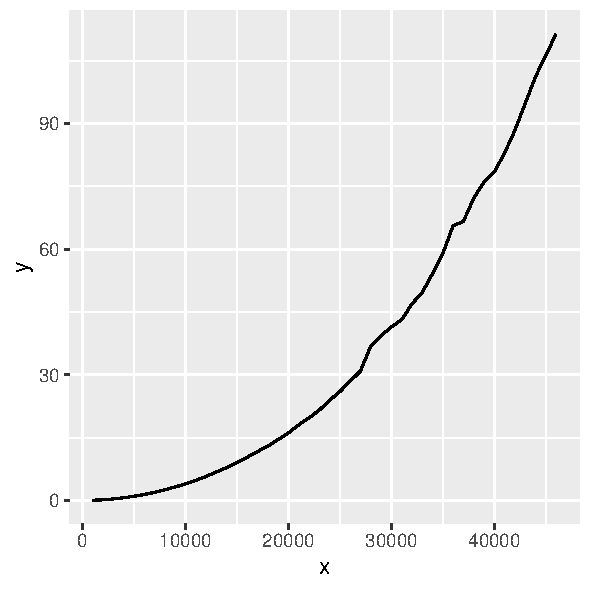
\includegraphics[width=10cm]{img/hclust}
	\caption{Time complexity of \texttt{hclust} with respect to the size of a dataset.}
	\label{fig01:hclust}
\end{figure}

Fig. \ref{fig01:hclust} supports the above stated polynomial time complexity of the implementation. Moreover, it stopped at a dataset size of 47K because the testing machine \footnote{Intel Core i9-8950HK, 32GB RAM} ran out of memory.

In conclusion, the space complexity of HCA can be even more restrictive in the means of the overall algorithm usability than its time complexity. The performance and usability of the HCA variants depends on many factors and the programmer needs to find a balance between their tradeoffs. The metric function is one of them. For example, when the Minkowski distance is used, we can prefer the in-place HCA over the HCA with dissimilarity matrix for a lower space complexity while retaining the same asymptotic time complexity. However, if the distance metric is more complex, one may prefer to store the measures in the memory.

